\documentclass{cshonours}
\usepackage{url}
\usepackage{graphics}
\usepackage{bibunits}
\usepackage{abbrevs}
\usepackage{acronym}
\usepackage[vario]{fancyref}
%\usepackage{gnuplot-lua-tikz}
\usepackage{xspace}
\usepackage{hyperref}

%%% BEGIN LATEX TWEAKS

% Hyperref setup
\hypersetup{hidelinks}

% Configure bibliography
\bibliographystyle{acm}
\defaultbibliography{../references/primary}
\defaultbibliographystyle{acm}

% Acronyms for common stuff
\newcommand{\acrodefn}[3]{%
	\acrodef{#1}[#2]{#3}%
	\expandafter\newcommand\csname#1\endcsname{\ac{#1}\xspace}%
}
\acrodefn{aecl}{AECL}{Atomic Energy Canada Limited}
\acrodefn{cgr}{CGR}{Compagnie General Radiographique}
\acrodefn{fda}{FDA}{U.S. Food and Drug Administration}
\acrodefn{maude}{MAUDE}{Manufacturer and User Facility Device Experience Database}
\acrodefn{soup}{SOUP}{Software of Unknown Pedigree}
\acrodefn{iso}{ISO}{International Standards Organisation}
\acrodefn{iec}{IEC}{International Electrotechnical Commission}
\acridefn{aami}{AAMI}{Association for the Advancement of Medical Instrumentation}

% Abbreviation commands for common stuff
% TODO: Fix spacing problem
\newabbrev\ther{Therac-25}
\newabbrev\etal{et al.}

% Fancyref support for subsections, source; https://github.com/openlilylib/tutorials/blob/master/aGervasoni/orchestralScores/example-materials/OLLbase.sty
\newcommand*{\fancyrefsubseclabelprefix}{subsec}

\fancyrefaddcaptions{english}{%
  \providecommand*{\frefsubsecname}{subsection}%
  \providecommand*{\Frefsubsecname}{Subsection}%
}

\frefformat{plain}{\fancyrefsubseclabelprefix}{\frefsubsecname\fancyrefdefaultspacing#1}
\Frefformat{plain}{\fancyrefsubseclabelprefix}{\Frefsubsecname\fancyrefdefaultspacing#1}

\frefformat{vario}{\fancyrefsubseclabelprefix}{%
  \frefsubsecname\fancyrefdefaultspacing#1#3%
}
\Frefformat{vario}{\fancyrefsubseclabelprefix}{%
  \Frefsubsecname\fancyrefdefaultspacing#1#3%
}


%%% END LATEX TWEAKS


\title{Therac-25:\\Will history repeat itself?}
\author{Ash Tyndall}

\begin{document}
\maketitle

\tableofcontents

\chapter{Introduction}

In the early 1970s, two companies, \aecl and \cgr, collaborated to build updated models of their core radiotheraputic offerings; Medical Linear Accelerators (LINACs). LINACs are an extension of the basic concept of a linear particle accelerator, repackaged for medical applications. They are are designed to create a beam of either electron or x-rays which can be focused on a very specific section of a patients body. These beams can be used to kill cancerous growths without severely damaging surrounding tissue.

Together, \aecl and \cgr develop two LINACs; the Therac-6 and the Therac-20, both of which were based on previous \cgr work, but with mechanical control substituted with control via computer terminal. These machines are designed with accelerators that could produce 6 MeV x-rays and 20 MeV x-rays/electrons respectively. Still in partnership in the mid-1970s, \aecl and \cgr develop a new Therac that uses a new kind of linear accelerator, a ``double-pass'' system, which reduces the space requirements and allows cheaper parts to be used. \aecl and \cgr part ways soon thereafter, citing competitive pressures. 

\aecl proceeded with the development of this new ``double-pass'' system, the \ther (so named for its 25 MeV x-ray and electron beam), continuing to develop the software-based control system, and passing the necessary regulatory requirements. The system is announced for public sale in 1983. One of the cutting-edge features of the machine is the removal of hardware-based interlocks and safeguards on the device, \aecl instead opting to use a wholly software-based approach to ensure that the appropriate components are rotated in front of the raw electron beam to reduce the dangerous radiation to therapeutic levels.

In 1985, the first reported case of \ther software safeguard failure occurred. Katherine Yarbrough, a breast cancer patient, receives an estimated 15,000--20,000 rads instead of the normal 200 rad range. She suffers severe radiation burns and shoulder and arm paralysis. A month later at a different facility, an unidentified female patient receives four separate overdoses totalling 13,000--17,000 rads within the space of several minutes, due to a combination of safeguard failure and poorly explained error messages. This patient dies of radiation induced cancer some months later.

It was initially unclear to those who operated the \ther that software errors were the cause of these overdoses. Due to the nature of radiation overdoses, the most serious of symptoms appear days if not weeks later, causing the resulting deaths and disablements to be attributed to other factors. However, over time, it became clear to different system operators that something was seriously wrong with the \ther, sparking an eventual forced FDA recall of the product with a total of six overdoses and two deaths.

% TODO: Cite
\ther was responsible for the first known deaths in radiotherapy, a profession that began some 35 years prior, and the confluence of death and computing caused an uproar at the time. Since then, the flames of anger have died down, and there is an opportunity to review the incident objectively. This report will examine the \ther case in detail, trying to determine the answers to several important questions:
\begin{enumerate}
 \item How does one design safe software, what does it involve, what are the pitfalls and how do we avoid them? (\Fref{chap:safesoftware})
 \item What were the flaws of \ther and how did failures on the part of \aecl and \cgr contribute to the creation of these flaws? (\Fref{chap:flawsfailures})
 \item How did standards and regulatory bodies respond to \ther through new guidelines and processes for creation of ``safe'' medical device software? (\Fref{chap:newstandards})
 \item Have those guidelines and processes resulted in the creation of safer medical device software? (\Fref{chap:data}) 
 \item Are there still areas in the medical landscape where regulation is insufficient? (\Fref{chap:reggaps})
 \item Will a disaster like \ther happen again? (\Fref{chap:conclusion})
\end{enumerate}

% TODO: Economic consequences of human death

\chapter{Literature Review}
\label{chap:litreview}
\ther was one of the first widely reported software-related disasters, and as a result, a variety of academic work has been performed since the disaster investigating the specifics of the failure of \ther, as well as the development of safety critical  medical software generally.

Primary work in the area of safety critical software development and system design as been done by Nancy Leveson. Her two books \textit{Safeware} \cite{safeware} and the more recent \textit{Engineering a Safer World} \cite{saferworld} are highly influential works in the field. They discuss from a variety of disciplines the causes of safety-critical system failure, from poor software testing processes to a failure of system design to adequately inform the user of the system's state. Of particular relevance to our \ther questions is \textit{Safeware} chapter 6, ``The Role of Humans in Automated Systems'', which describes several models of human-computer interaction and the necessary design principles to properly enable them. Additionally, \textit{Engineering a Safer World} chapter 9, ``Safety-Guided Design'', which discusses several of the \ther design flaws.

Leveson and Turner have also contributed the primary academic report on \ther \cite{leveson1993investigation} which discusses the history of the Therac brand, the history of the companies involved, as well as the timeline of the disasters that ensued.

Various work has been done into the area of safe critical software from both the perspective of cause and prevention. Dunn \cite{dunn2003designing} provides us with a helpful definition of safety in terms of ``mishap risk'', as well as examples of mishap causes.

In terms of cause, in \textit{Failure in Safety-Critical Systems} \cite[ch.~3]{johnson2003failure} Johnson discusses in detail the sources of failure, touching upon a broad variety of failures including Regulatory, Managerial, Hardware, Software, Human and Team based failures. Besnard and Baxter \etal \cite{besnard2003human} discuss two models of system failure, Reason's swiss cheese model and Randell's fault-error-failure model, both of which can be used to analyse the \ther disaster.

In terms of prevention, Nolan \cite{nolan2000system} proposes several strategies to be considered when designing ``safe systems of care'', as well as methods to reduce ``adverse events''  which may compromise patient health. Obradovich and Woods \cite{obradovich1996users} perform an investigation of poor Human-Computer Interface design in a medical device, describing how the device is flawed and how both the user and medical supervisor can change their processes to cope with this. Lin, Vicente and Doyle \cite{lin2001patient} propose a new interface for a specific medical appliance that applies human factors engineering, a key part of the discussed prevention of user error, and provides data demonstrating the effectiveness of such an approach from error minimisation and efficiency perspectives.

Several works discuss the introduction of various international standards and regulations post-\ther. Rakitin \cite{rakitin2006coping} provides an overview of foundational standards in the risk management space of medical device software. Brown \cite{brown2000overview} provides an overview of specifically the IEC 61508 ``Design of electrical / electronic / programmable electronic safety-related systems'' standard. Jordan \cite{jordan2006standard} provides an overview of specifically the IEC 62304 ``Medical Device Software -- Software Lifecycle Processes'' standard.

To allow us to determine if regulation of medical device software has improved the situation, several works which analyse relevant data will be examined. Wallace and Kuhn produced two papers \cite{wallace1999lessons,wallace2001failure} analysing a subset of \fda data relating to ``adverse events'' and provided statistics on the types of software errors and the medical domain of the devices, as well as information on how to prevent and detect these types of errors. The \fda \maude dataset \cite{maude} is also examined directly by the author to attempt to derive conclusions regarding the proportion of medical device software errors in the broader \maude database. Finally, \textit{Failure in Safety-Critical Systems} \cite[ch.~5]{johnson2003failure} discusses the under-reporting of incidents, as well as reporting bias.

\chapter{Safe software design:\\What does it involve?}
\label{chap:safesoftware}
The design of safe software (or as Leveson calls it, ``Safeware'' \cite{safeware}) is of paramount importance in the medical industry, as the software is frequently placed in direct control of equipment that has the potential to serious injure or kill if it operates outside (usually thin) safety margins. In the case of \ther, the machine was capable in certain failure states of emitting radiation that was able to cause death and permanent disablement.

It is difficult however to define what exactly ``safety'' is; granted, we can say that a system is ``safe'' if there is absolutely no chance that anything could go wrong with it, however, such systems do not exist in the real world. Dunn \cite{dunn2003designing} touches upon a useful concept to consider safety; a safe system is one with an acceptably low ``mishap risk''. Dunn uses the US Department of Defence definition of mishap; ``an unplanned event or series of events that result in death, injury, occupational illness, damage to or loss of equipment or property, or damage to the environment.'', suggesting that mishap risk deals with the impact or severity of a given mishap event, and the probability of it occurring. Another common team in the medical field that could be considered a synonym with mishap is ``adverse event'', which is more specifically and generally defined as ``any undesirable experience associated with the use of a medical product in a patient.'' \cite{fdaadverse}

Since \ther, much discussion has taken place on strategies to mitigate ``adverse events'' involving medical device software. Leveson argues that safe software design can only be achieved through creation of both a culture of safety, \cite[ch.~4]{safeware} and embedding Safeware design principles into the software from the beginning \cite[ch.~16]{safeware}. She argues that it is not enough to identify how a system can go wrong, but also institute changes that make those occurrence less likely by design. A strong culture of safety also ensures that complacency regarding safety, safety-apathetic organisational structures and lack of technical skill in implementing and ensuring safety in product are not present, which Leveson argues are key causes of software disaster.

Safeware design principles concern themselves primarily with hazard reduction as a primary goal and consideration when designing software. Leveson notes that in many industries outside of software, there exists a large body of knowledge; standards, codes of practice and checklists, which provide a large degree of guidance to the design of physical products with safety consideration. However, such codes are present to a lesser extent in software, and mainly concern themselves with concepts of readability and complexity, rather than ``safe'' architecture.

Within software, Leveson proposes four ways to reduce accidents through design changes. The first of these is hazard elimination, involving preventing hazards through design by making them physically impossible. Some possible hazard elimination methods include;
 \begin{itemize}
  \item \textbf{Substitution}; change components with hazardous effects with others
  \item \textbf{Simplification}; simply design such that hazards caused by complex interactions are removed
  \item \textbf{Decoupling}; reduce adverse effects of unexpected behaviour in a subsystem by making it only loosely coupled with other systems
  \item \textbf{Elimination of specific human error}; reduce obvious error by making system status unambiguous and easy to understand
  \item \textbf{Reduction of hazardous materials or conditions}; ensure software only contains code necessary for core functionality, remove unused code
 \end{itemize}
 
The second of these is hazard occurrence reduction, whereby the probability of a hazard occurring is reduced, such as by;
 \begin{itemize}
  \item \textbf{Design for controllability}; provide feedback about system state while critical actions occur, provide operator time to react to perceived problems with system
  \item \textbf{Barriers}; erect physical or logical barriers between safe and unsafe tasks, unsafe tasks should not be easy to do accidentally
  \item \textbf{Failure minimisation}; ensure safety factors and margins, as well as redundancy
 \end{itemize}
 
The third of these is hazard control, through which the probability of a hazard leading to an accident can be reduced through a variety of methods;
 \begin{itemize}
  \item \textbf{Limiting exposure}; critical software checks should be as close in execution as the code they protect, critical checks should also not be complimentary
  \item \textbf{Isolation and containment}; the number of people who could be affected by a hazard should be reduced to as low as practical
  \item \textbf{Protection systems and Fail-safe design}; independent watchdog hardware can be introduced to ensure that a failed system is returned back to a safe state
 \end{itemize}

The final of these is damage reduction. Potential hazards need to be understood, and emergency plans and training to handle these hazards should they arise should be provided to relevant people such than in the case of an hazard-caused accident, damage mitigating action can occur.

Leveson's proposed accident reduction techniques can be though of in terms of Besnard and Baxter's \cite{besnard2003human} integration of Reason and Randell's swiss-cheese and fault-error-failure models, shown in \Fref{fig:besnardmodel}. In this diagram we can see that the first three of Leveson's proposed accident reduction techniques serve as barriers through which adverse events cannot traverse, but though the introduction of faults in these layers, errors are able to arise that eventually become failures that cause holes in these barriers. If these barriers happen to be broken in the same area, it can lead to accidents, harm and loss of life. Safe software design involves instituting processes that ensure that as little faults are introduced into these barriers as possible.

\begin{figure}
 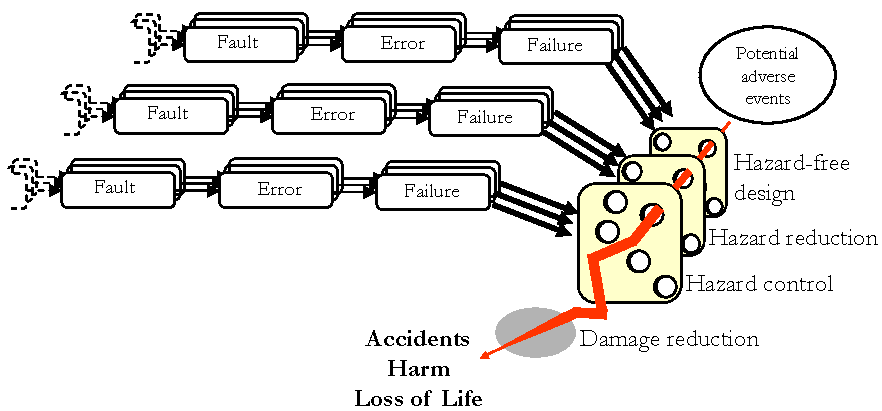
\includegraphics[width=\textwidth]{figs/besnardmodified.pdf}
 \caption{Model of Leveson's hazard reduction (adapted from \cite[fig.~6]{besnard2003human})}
 \label{fig:besnardmodel}
\end{figure}

Lin \cite{lin2001patient} provides a study of medical device interfaces which we can apply Leveson's proposed principles to investigate their effectiveness. In her study the user interface of a specific medical device, designed to administer specific quantities of a drug, was analysed against a proposed user interface which better applied Human-Computer Interface principles. This interface rearranged the design of the buttons used to input data, as well as changed the graphics displayed when navigating the device to give the user a much better sense of the implications of their actions, as well as the current mode of the machine. This could be considered a form of hazard elimination due to design; by reducing the confusion between the user's actions and the results, hazards related to erroneously entered parameters is greatly reduced. When statistically comparing the use of the old interface and the new interface, Lin noted an average reduction of error of 44\%.

Lin's changes to the interface were not drastic, but clearly demonstration how a safety orientated approach can be quite effective in preventing error.


\chapter{Flaws and failures:\\How and why?}
\label{chap:flawsfailures}
The \ther incidents are generally used as a case-study in literature on safety-critical devices, as they serve as very good example of a failure of software processes and ``safeware'' at multiple levels. As such, extensive investigation on the many facets of those failures exists, and a variety of research exists exploring the incident at multiple levels. Here we'll discuss some of the reasons \ther failed from a management and process perspective, as well as touching upon how some failures of user interface design exacerbated these errors.

The primary software error present in \ther was a race condition, triggered if the operator were to perform steps 3 and 4 of the following within 8 seconds;
\begin{enumerate}
 \item Press ``X'' to select X-ray in the Mode field.
 \item Press the ``Up'' arrow to re-position the cursor on the Mode field.
 \item Press ``E'' to change the selection to Electron mode.
 \item Press ``Enter'' to submit all other values unchanged and trigger the dispensing of radiation.
\end{enumerate}
This race condition existed due to a hard-coded timer 

The ultimate failure of \ther was the lack of safety as a primary consideration in the software development and design process. As described by Leveson and Turner in their investigation of the incident \cite{leveson1993investigation} little documentation was kept regarding the specifications of the software running \ther, nor on the testing process to ensure that the safety of the system was maintained. Software testing was only considered as part of broader whole-system tests, which would make complex software flaws much more difficult to find and fix. Furthermore, the software was developed by only one individual, leading to important questions about the amount of oversight that existed over the software quality and design. It is evident that \aecl's management either did not have the will or the competence to ensure the thorough testing of the \ther system, and a emphasis safety goals generally, with studies indicating that such an emphasis is one of the strongest indicators of a safe system. \cite[p.~415]{saferworld}

One of the serous process issues uncovered as part of the \ther investigation was the fact the software used in \ther was partially ported from the prior Therac-6, which while architecturally similar, contained electromechanical safeguards in addition to software based ones. With \aecl's track record with documentation in serious question, the Therac-6 software could rightly be considered \soup, as without extensive specific software testing having been performed on the Therac-6, one could not rightly assume that the Therac-6 software is free of bugs that could have adverse safety implications. It was later determined that one of the primary bugs responsible for the \ther deaths was also present in Therac-20, but due to the hardware safeguards, merely caused the machine to shut down, suggesting the bug may have partial genesis in this use of \soup.

Another serious issue with process was the near complete exclusion of software from core safety analysis steps of the \ther system, to quote \aecl's final report; 
\begin{quote}
Programming errors have been reduced by extensive testing on a hardware simulator and under field conditions on teletherapy units. Any residual software errors are not included in the analysis. \cite[p.~4]{leveson1993investigation}
\end{quote}
In that same report, \aecl assigns extraordinarily low probabilities to errors such as ``Computer selects wrong mode'' ($4 \times 10^{-9}$). This betrays \aecl's attitudes towards software safety, and their failure to consider the dangers of using \soup within their products. 

It is also illuminating to analyise the \ther disaster from the perspective of software design as a whole. Leveson \cite{safeware} provides several useful frameworks through which to analyse both a user and a computer's role within a given system. These are X, Y, Z (TODO: FILL IN). The most applicable of these to \ther would be human as monitor; a system in which the computer itself is responsible for the executive actions in the system, and the human serves a supervisory role, ensuring that the process is error free. This may seem at odds when considering the entire intelligence of the system being still vested in the human, however the actual execution of the actions are the sole domain of the computer system. Leveson goes on to discuss how in such a system, it is important that for the human to be sufficiently aware of the system's state to be an effective monitor; ``[t]he operator is dependent on the information provided; it is easy to provide too much or too little information or to display it poorly,.'' \cite[p.~TODO]{safeware} \ther failed to provide appropriate levels of information in several ways;
\begin{enumerate}
  \item Error messages were vauge with description, with the details contained within unexplained numerical codes, making it impossible for the operator to know specifically what was wrong. E.g. ``Error 1''.
  \item Both dangerous and benign failures were represented by the same error code, habituating operators to ignoring them.
\end{enumerate}

\ther is also a useful case study in counter-productive Human-Computer Interface (HCI) design. The system, for reasons of safety, required that parameters be entered multiple times, and if these entries mismatched, then an error would display and the treatment would not proceed. However, this ended with complaints from operators for arduousness, thus it was augmented with a system whereby the user could press Enter to confirm that a parameter set was correct. While efficient, this had the net result of habitualising the operators to press Enter in quick succession, thus reducing the safety gained from requiring careful consideration of the parameters. \cite[p.~274]{saferworld}

A similar HCI issue involved the ``Treatment Pause'' functionality, which allowed an operator to continue with treatment of a patient after recieving an error message up to five times before necessitating a system reboot. Due to the aforementioned poor error messages, this simply lead to the habitualization of operators resuming treatment in the case of error, as in the vast majority of circumstances, this would have no ill effect. \cite[p.~301]{saferworld}

Ultimately it is difficult to pin down who at \aecl was responsible for the lack of appropriate safety culture, as subsequent lawsuits and regulatory investigations disincentivise parties with information from speaking out. However, due to the scale of the incident and the public nature of those lawsuits that did occur, enough information does exist to point to broad causes for the failure.
\cite{

\chapter{Regulatory response:\\New standards}
\label{chap:newstandards}
In September 1987, two years after the first recorded \ther radiation overdose, the \fda announced that they intended to introduce regulations to prevent the failures of software quality management that had been present in \aecl. \cite{jacky1989programmed} The following two decades saw the introduction of a variety of international standards to deal with the various facets of medical device software safety. These regulations are not necessarily easily unified, to quote one attempt at doing so; ``with so many different standards, regulatory guidance papers and industry guides on RM [risk management], the task of collating this information into a usable model is itself daunting.'' \cite{burton2006risk} To reasonbly restrict scope, only prominent United State national and international regulation from standards bodies regarding safe software development will be covered here.

Before the introduction of the first international standards, it was the sole job of the \fda to regulate medical device hardware within America. Information from this period is difficult to find, however, Leveson does mention the introduction of mandatory reporting by health-care facilities of adverse events in 1990. \cite[p.~TODO]{safeware}  This added to the preexisting requirements of manifacturers and importers to report such events.

One of the first international standards in this area that could potentially apply to medical device software is \textit{IEC 61508: Functional Safety of Electrical/Electronic/Programmable Electronic Safety-related Systems}, the first portions of which were published by the \iec in 1998. This standard provides a general set of standards creating a safety life cycle that can be adapted for specific industries. Notably, unlike \ther, it recognised that software risk cannot be reduced to zero, it can only be reduced, and as Leveson suggests, safety considerions must be present at every stage of the development lifecycle. \cite{brown2000overview} Jordan suggests however that the application of this standard to the medical area is difficult, as the area inherently has high risk, and the standard is most effective when dealing with low risk environments. \cite{jordan2006standard} 

In the same year, the \iso released their own standard specifically relating to medical device risk management; \textit{ISO 14971: Medical devices -- Application of risk management to medical device}. One of the key features of this standard was the requirment of evidence to exist in documentation that mitigation of risk in software was present, one of the key failings of \aecl. \cite{rakitin2006coping}

In 2000, a revision to parts 1--4 of \texit{IEC 60601: Medical Electrical Equipment} was released, which assisted in defining risk management more clarely, and adopted a defition of ``mishap risk'' that recognised both the severity and the probability of an issue. \cite{rakitin2006coping}

In 2001, the \aami in association with the American National Standards Institute released \textit{AAMI SW68: Medical device software - Software life cycle processes} which extended the risk management attributes ISO 14971 info a whole software development life cycle. \cite{rakitin2006coping} Burton, Mc Caffery and Richardson discuss how both ISO 14971 and AAMI SW68 were deficient in that they required risk management processes to be in place, but did not provide any specifics. \cite{burton2006risk}

In 2004, \texit{AAMI TIR32: Medical Device Software Risk Management} was published, which aimed to address the aforementioned deficiencies of ISO 14971 and AAMI SW68 by clarifying the risk management processes. \cite{rakitin2006coping} In particular, it provided clear definitions of reliability and safety, and importantly how they differ;
\begin{quote}
Reliability is the ability of a system to perform its required functions under stated conditions for a specified period of time. Safety is the probability that conditions (hazards) that can lead to a mishap do not occur, whether or not the intended function is performed. Reliability is interested in all possible software errors, while safety is concerned only with those errors that cause actual system hazards. \cite{aamitir32}
\end{quote}

Finally, in 2006, the \iec published the most recent standard in the area, \textit{IEC 62304: Medical device software -- Software life cycle processes}, which determines those processes, activities and tasks that are necessary for the creation of dependably and reliably medical device software. Huhn and Zechner note however that no specific models nor methods are perscribed to accompish these tasks, the manifacturer must instead argue that their own processes allow for the creation of such dependable and reliable medical device software. \cite{huhn2010arguing} Jordan suggests that in the industry, such processes, activities and tasks are already core to reputable manufacturers, thus the lack of perscrition is welcome to them. \cite{jordan2006standard}


\chapter{Data analysis:\\Are we safer?}
\label{chap:data}
While the discussion of regulation is useful, it is hard to say to what extent that has resolved the safety issues in medical device software that \ther demonstrated. Have regulators appropriately determined what is necessary to ensure these bugs are minimal? Is it possible to create software that has sufficiently low ``mishap risk'' in this realm?

\section{MAUDE}
There are several data sets that could potentially provide answers to these questions. The first of these is the \fda's \maude, a massive database of adverse events reported to the \fda available for download on their website. This dataset extends from the year 2000 to the current day.

\maude data consists of information relating to each adverse event including the manufacturer involved, the device involved, the category of adverse event and a free-form text field which contains further description from the manufacturer about the nature of the issue.

Using the \maude database, it may be possible to measure the proportion of issues manufacturers have reported as being related to medical device software in some form. From those statistics, it may be possible to derive trends, such as if device software is becoming more or less safe. The most useful data attribute for such a purpose is clearly the category: the \fda provides an extensive (nearly 1,000) list of categories, to one of which each adverse event can be assigned.

The first analysis on \maude involved determining a list of categories considered relevant to medical device software adverse events, and then querying the database to determine what proportion of adverse events each year were contained within that category. 

The categories chosen for that purpose were;
\begin{itemize}
  \item Computer failure
  \item Computer hardware error
  \item Computer software issue
  \item Incorrect display
  \item Error or warning message, failure to produce
  \item Power calculation error due to software problem
  \item Incorrect software programming calculations
  \item Algorithms, inconsistent
  \item Semiautomatic code, failure to override
  \item Year 2000 (Y2K) related problem
  \item Date-related software issue
  \item Application network issue
  \item Application program issue
  \item Application program version or upgrade problem
  \item Application security issue
  \item Computer operating system issue
  \item Computer system security issue
  \item Data back-up problem
  \item Loss of Data
  \item Operating system becomes non-functional
  \item Operating system version or upgrade problem
  \item Problem with software installation
  \item Programming issue
\end{itemize}

The database was analysed, with the proportion of software events never becoming greater than 0.4\%. \Fref{fig:proportiongraph} shows the proportion of incidents of the above categories within the larger database. Upon analysing the data in this database, it is difficult to come to any complete conclusions about these proportions. Before 2007, there are no adverse events corresponding to those categories in \maude, suggesting that either those categories were either non-existent, or the introduction of categories entirely was introduced in that year. From 2007--12, there are less than 10 reports matching the medical device software categories, suggesting that those categories are not readily used. 2013--14 shows significantly more of these categories, but they do not alone provide enough data points to draw any conclusions.

Furthermore, it appears that the pubicly accessible data within \maude is only a recently phenomenom, with \Fref{fig:totalgraph} showing how the public data present increases massively over the period covered.

\begin{figure}
  \begin{tikzpicture}[gnuplot]
%% generated with GNUPLOT 4.6p4 (Lua 5.1; terminal rev. 99, script rev. 100)
%% Tue 21 Oct 2014 14:08:55 WST
\tikzset{every node/.append style={font={\fontsize{9pt}{10.8pt}\selectfont}}}
\gpmonochromelines
\path (0.000,0.000) rectangle (12.700,7.620);
\gpcolor{color=gp lt color border}
\gpsetlinetype{gp lt border}
\gpsetlinewidth{1.00}
\draw[gp path] (1.356,0.886)--(1.536,0.886);
\draw[gp path] (12.201,0.886)--(12.021,0.886);
\node[gp node right] at (1.190,0.886) {0};
\draw[gp path] (1.356,1.686)--(1.536,1.686);
\draw[gp path] (12.201,1.686)--(12.021,1.686);
\node[gp node right] at (1.190,1.686) {0.05};
\draw[gp path] (1.356,2.486)--(1.536,2.486);
\draw[gp path] (12.201,2.486)--(12.021,2.486);
\node[gp node right] at (1.190,2.486) {0.1};
\draw[gp path] (1.356,3.286)--(1.536,3.286);
\draw[gp path] (12.201,3.286)--(12.021,3.286);
\node[gp node right] at (1.190,3.286) {0.15};
\draw[gp path] (1.356,4.087)--(1.536,4.087);
\draw[gp path] (12.201,4.087)--(12.021,4.087);
\node[gp node right] at (1.190,4.087) {0.2};
\draw[gp path] (1.356,4.887)--(1.536,4.887);
\draw[gp path] (12.201,4.887)--(12.021,4.887);
\node[gp node right] at (1.190,4.887) {0.25};
\draw[gp path] (1.356,5.687)--(1.536,5.687);
\draw[gp path] (12.201,5.687)--(12.021,5.687);
\node[gp node right] at (1.190,5.687) {0.3};
\draw[gp path] (1.356,6.487)--(1.536,6.487);
\draw[gp path] (12.201,6.487)--(12.021,6.487);
\node[gp node right] at (1.190,6.487) {0.35};
\draw[gp path] (1.356,7.287)--(1.536,7.287);
\draw[gp path] (12.201,7.287)--(12.021,7.287);
\node[gp node right] at (1.190,7.287) {0.4};
\draw[gp path] (1.356,0.886)--(1.356,1.066);
\draw[gp path] (1.356,7.287)--(1.356,7.107);
\node[gp node center] at (1.356,0.609) {1994};
\draw[gp path] (2.441,0.886)--(2.441,1.066);
\draw[gp path] (2.441,7.287)--(2.441,7.107);
\node[gp node center] at (2.441,0.609) {1996};
\draw[gp path] (3.525,0.886)--(3.525,1.066);
\draw[gp path] (3.525,7.287)--(3.525,7.107);
\node[gp node center] at (3.525,0.609) {1998};
\draw[gp path] (4.610,0.886)--(4.610,1.066);
\draw[gp path] (4.610,7.287)--(4.610,7.107);
\node[gp node center] at (4.610,0.609) {2000};
\draw[gp path] (5.694,0.886)--(5.694,1.066);
\draw[gp path] (5.694,7.287)--(5.694,7.107);
\node[gp node center] at (5.694,0.609) {2002};
\draw[gp path] (6.779,0.886)--(6.779,1.066);
\draw[gp path] (6.779,7.287)--(6.779,7.107);
\node[gp node center] at (6.779,0.609) {2004};
\draw[gp path] (7.863,0.886)--(7.863,1.066);
\draw[gp path] (7.863,7.287)--(7.863,7.107);
\node[gp node center] at (7.863,0.609) {2006};
\draw[gp path] (8.948,0.886)--(8.948,1.066);
\draw[gp path] (8.948,7.287)--(8.948,7.107);
\node[gp node center] at (8.948,0.609) {2008};
\draw[gp path] (10.032,0.886)--(10.032,1.066);
\draw[gp path] (10.032,7.287)--(10.032,7.107);
\node[gp node center] at (10.032,0.609) {2010};
\draw[gp path] (11.117,0.886)--(11.117,1.066);
\draw[gp path] (11.117,7.287)--(11.117,7.107);
\node[gp node center] at (11.117,0.609) {2012};
\draw[gp path] (12.201,0.886)--(12.201,1.066);
\draw[gp path] (12.201,7.287)--(12.201,7.107);
\node[gp node center] at (12.201,0.609) {2014};
\draw[gp path] (1.356,7.287)--(1.356,0.886)--(12.201,0.886)--(12.201,7.287)--cycle;
\node[gp node center,rotate=-270] at (0.221,4.086) {\%};
\node[gp node center] at (6.778,0.194) {Year};
\gpcolor{color=gp lt color 0}
\gpsetlinetype{gp lt plot 0}
\draw[gp path] (1.898,0.886)--(2.441,0.886)--(3.525,0.886)--(4.067,0.886)--(4.610,0.886)%
  --(5.152,0.886)--(5.694,0.886)--(6.236,0.886)--(6.779,0.886)--(7.321,0.886)--(7.863,0.886)%
  --(8.405,3.659)--(8.948,2.874)--(9.490,6.238)--(10.032,3.105)--(10.574,4.847)--(11.117,3.151)%
  --(11.659,6.331)--(12.201,6.773);
\gpcolor{color=gp lt color border}
\gpsetlinetype{gp lt border}
\draw[gp path] (1.356,7.287)--(1.356,0.886)--(12.201,0.886)--(12.201,7.287)--cycle;
%% coordinates of the plot area
\gpdefrectangularnode{gp plot 1}{\pgfpoint{1.356cm}{0.886cm}}{\pgfpoint{12.201cm}{7.287cm}}
\end{tikzpicture}
%% gnuplot variables

  \caption{Proportion of incidents in medical device software related categories over time}
  \label{fig:proportiongraph}
\end{figure}

\begin{figure}
  \begin{tikzpicture}[gnuplot]
%% generated with GNUPLOT 4.6p4 (Lua 5.1; terminal rev. 99, script rev. 100)
%% Wed 08 Oct 2014 21:52:41 WST
\tikzset{every node/.append style={font={\fontsize{9pt}{10.8pt}\selectfont}}}
\gpmonochromelines
\path (0.000,0.000) rectangle (12.700,7.620);
\gpcolor{color=gp lt color border}
\gpsetlinetype{gp lt border}
\gpsetlinewidth{1.00}
\draw[gp path] (1.245,0.886)--(1.425,0.886);
\draw[gp path] (12.201,0.886)--(12.021,0.886);
\node[gp node right] at (1.079,0.886) {0};
\draw[gp path] (1.245,1.800)--(1.425,1.800);
\draw[gp path] (12.201,1.800)--(12.021,1.800);
\node[gp node right] at (1.079,1.800) {5000};
\draw[gp path] (1.245,2.715)--(1.425,2.715);
\draw[gp path] (12.201,2.715)--(12.021,2.715);
\node[gp node right] at (1.079,2.715) {10000};
\draw[gp path] (1.245,3.629)--(1.425,3.629);
\draw[gp path] (12.201,3.629)--(12.021,3.629);
\node[gp node right] at (1.079,3.629) {15000};
\draw[gp path] (1.245,4.544)--(1.425,4.544);
\draw[gp path] (12.201,4.544)--(12.021,4.544);
\node[gp node right] at (1.079,4.544) {20000};
\draw[gp path] (1.245,5.458)--(1.425,5.458);
\draw[gp path] (12.201,5.458)--(12.021,5.458);
\node[gp node right] at (1.079,5.458) {25000};
\draw[gp path] (1.245,6.373)--(1.425,6.373);
\draw[gp path] (12.201,6.373)--(12.021,6.373);
\node[gp node right] at (1.079,6.373) {30000};
\draw[gp path] (1.245,7.287)--(1.425,7.287);
\draw[gp path] (12.201,7.287)--(12.021,7.287);
\node[gp node right] at (1.079,7.287) {35000};
\draw[gp path] (1.245,0.886)--(1.245,1.066);
\draw[gp path] (1.245,7.287)--(1.245,7.107);
\node[gp node center] at (1.245,0.609) {1975};
\draw[gp path] (2.615,0.886)--(2.615,1.066);
\draw[gp path] (2.615,7.287)--(2.615,7.107);
\node[gp node center] at (2.615,0.609) {1980};
\draw[gp path] (3.984,0.886)--(3.984,1.066);
\draw[gp path] (3.984,7.287)--(3.984,7.107);
\node[gp node center] at (3.984,0.609) {1985};
\draw[gp path] (5.354,0.886)--(5.354,1.066);
\draw[gp path] (5.354,7.287)--(5.354,7.107);
\node[gp node center] at (5.354,0.609) {1990};
\draw[gp path] (6.723,0.886)--(6.723,1.066);
\draw[gp path] (6.723,7.287)--(6.723,7.107);
\node[gp node center] at (6.723,0.609) {1995};
\draw[gp path] (8.092,0.886)--(8.092,1.066);
\draw[gp path] (8.092,7.287)--(8.092,7.107);
\node[gp node center] at (8.092,0.609) {2000};
\draw[gp path] (9.462,0.886)--(9.462,1.066);
\draw[gp path] (9.462,7.287)--(9.462,7.107);
\node[gp node center] at (9.462,0.609) {2005};
\draw[gp path] (10.832,0.886)--(10.832,1.066);
\draw[gp path] (10.832,7.287)--(10.832,7.107);
\node[gp node center] at (10.832,0.609) {2010};
\draw[gp path] (12.201,0.886)--(12.201,1.066);
\draw[gp path] (12.201,7.287)--(12.201,7.107);
\node[gp node center] at (12.201,0.609) {2015};
\draw[gp path] (1.245,7.287)--(1.245,0.886)--(12.201,0.886)--(12.201,7.287)--cycle;
\node[gp node center] at (6.723,0.194) {Year};
\gpcolor{color=gp lt color 0}
\gpsetlinetype{gp lt plot 0}
\draw[gp path] (1.793,0.886)--(4.806,0.886)--(5.627,0.886)--(6.723,0.886)--(6.997,0.887)%
  --(7.545,0.887)--(7.819,0.886)--(8.092,0.887)--(8.366,0.889)--(8.640,0.890)--(8.914,0.912)%
  --(9.188,0.926)--(9.462,0.943)--(9.736,0.977)--(10.010,0.992)--(10.284,1.033)--(10.558,1.105)%
  --(10.832,1.150)--(11.105,1.477)--(11.379,1.661)--(11.653,3.842)--(11.927,6.852);
\gpcolor{color=gp lt color border}
\gpsetlinetype{gp lt border}
\draw[gp path] (1.245,7.287)--(1.245,0.886)--(12.201,0.886)--(12.201,7.287)--cycle;
%% coordinates of the plot area
\gpdefrectangularnode{gp plot 1}{\pgfpoint{1.245cm}{0.886cm}}{\pgfpoint{12.201cm}{7.287cm}}
\end{tikzpicture}
%% gnuplot variables

  \caption{Number of reports in \maude over time}
  \label{fig:totalgraph}
\end{figure}

% TODO: Other data stuff

\chapter{Regulatory gaps:\\What's next?}
\label{chap:reggaps}


\chapter{Conclusion:\\Will history repeat?}
\label{chap:conclusion}


\appendix

\bibliography{primary}

\end{document}